\newpage
\section{New Public Transport Technologies}
\label{sec:newtech}
In this paragraph, as previously stated, we are going to analyze the public transport future requirements that, in term of technologies, are becoming increasingly stringent. In order to be competitive on the bus market, the vehicles have to be equipped with a lot more technologies than nowadays. The technologies are needed since the world now is demanding more an more data and insights on every activity, not only from a generic and distant point of view, but from a direct, punctual and real-time view. Nowadays Public Transport in Italy, and buses in particular, are often equipped with close to nothing technologies that can improve the service; as we have seen in the previous chapters, Arriva systems used to collect the data in a quite old way: all the spreadsheets concerning the service, control management, balance sheets are clearly written by hand.

Public Transport technology innovation is not just the systems that can be installed onboard, such as the AVL or APC, but also all the world that revolve around them, from the service’s planning and management to the data gatherings and costumer feedbacks. All the innovative technology can be divided in two big groups: the systems that are installed directly on the buses, and the systems that operate remotely, off the buses.


\subsection{Technologies installed on bus}
\label{subsec:techonbus}

\begin{figure}[h!]
    \centering
    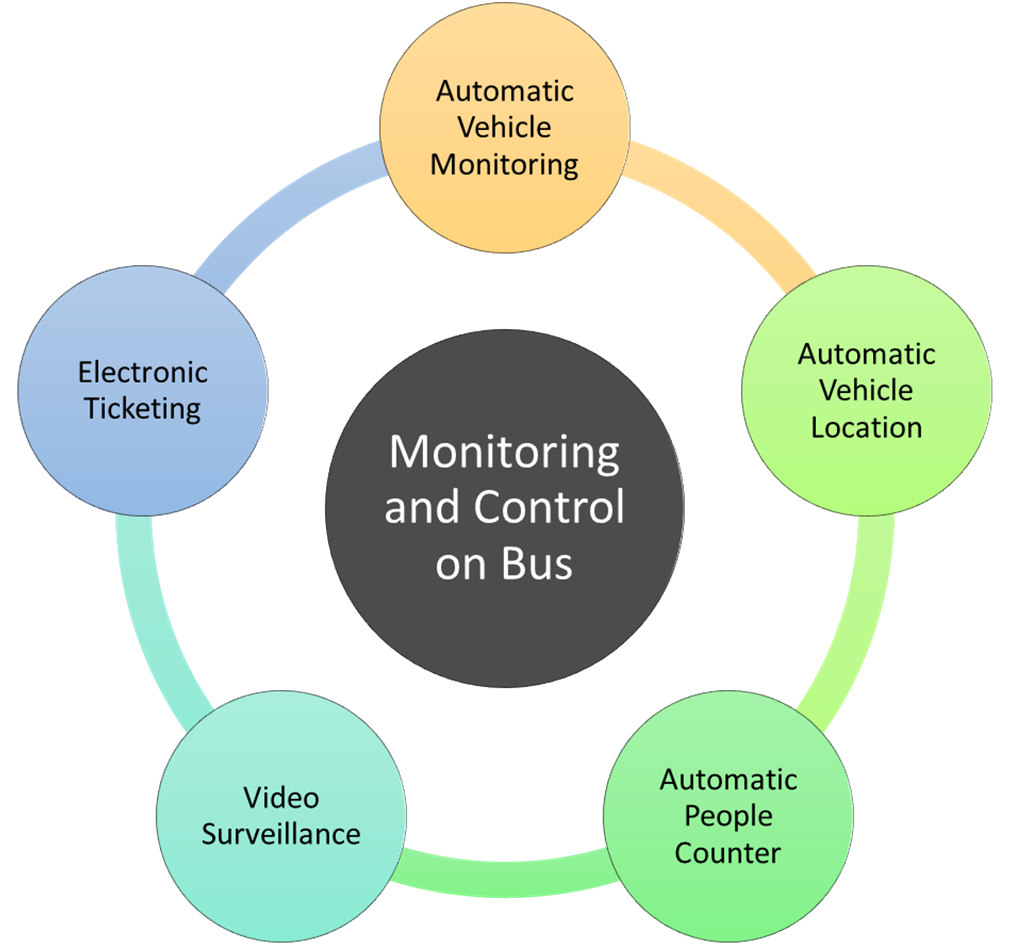
\includegraphics[width=0.4\textwidth]{Images/New Technologies/immagine intro Tech On.png}
    \caption{Technology Installed on Bus}
    \label{fig:onbus}
\end{figure}


The purpose of on – bus technology is mainly service monitoring and data gathering for demand analysis and offer adjustments, those type of system have become particularly relevant in the, very recent, Covid–19 period where it was particularly relevant analyze and report the mobility evolution to prospect near future scenarios and assess the effectiveness of adopted actions.


\paragraph{AVM and AVL}
Automated Vehicle Monitoring is a technology based on localization through GPS, monitoring and recording different topics related to moving vehicles, such as position, speed, diagnostic of mechanical components and so on. Automated Vehicle Location is more focused on the GPS position on the vehicle but if GPS signals are poor, AVL can use different technologies to determine actual location information, such as dead reckoning, which takes a previously determined position, and then incorporates estimations of speed, heading direction, and course over elapsed time. 

The buses, based on the GPS signal that the satellite sends, calculate their position a certain amount of seconds. This information, together with other data, is sent to the operator in the operation centre which operate in real-time the data and sends them to the costumer information management systems. Those data are also stored in order to make them available to the procuring entity for service reporting.

This type of technology allow the PTO to increase the security level and control in case of disruptive events, being able to handle and analyze big amount of data to assess a quick result or motivation.

Those technologies can be used to compute some interesting KPIs, tacking the status of the service, advances and delays, vehicle tracking, service adjustments in case of disruptive events. Also, from a graphical point of view the real-time situation can be displayed really well and it can be used widely in a dashboard.
\begin{figure}[H]
    \centering
    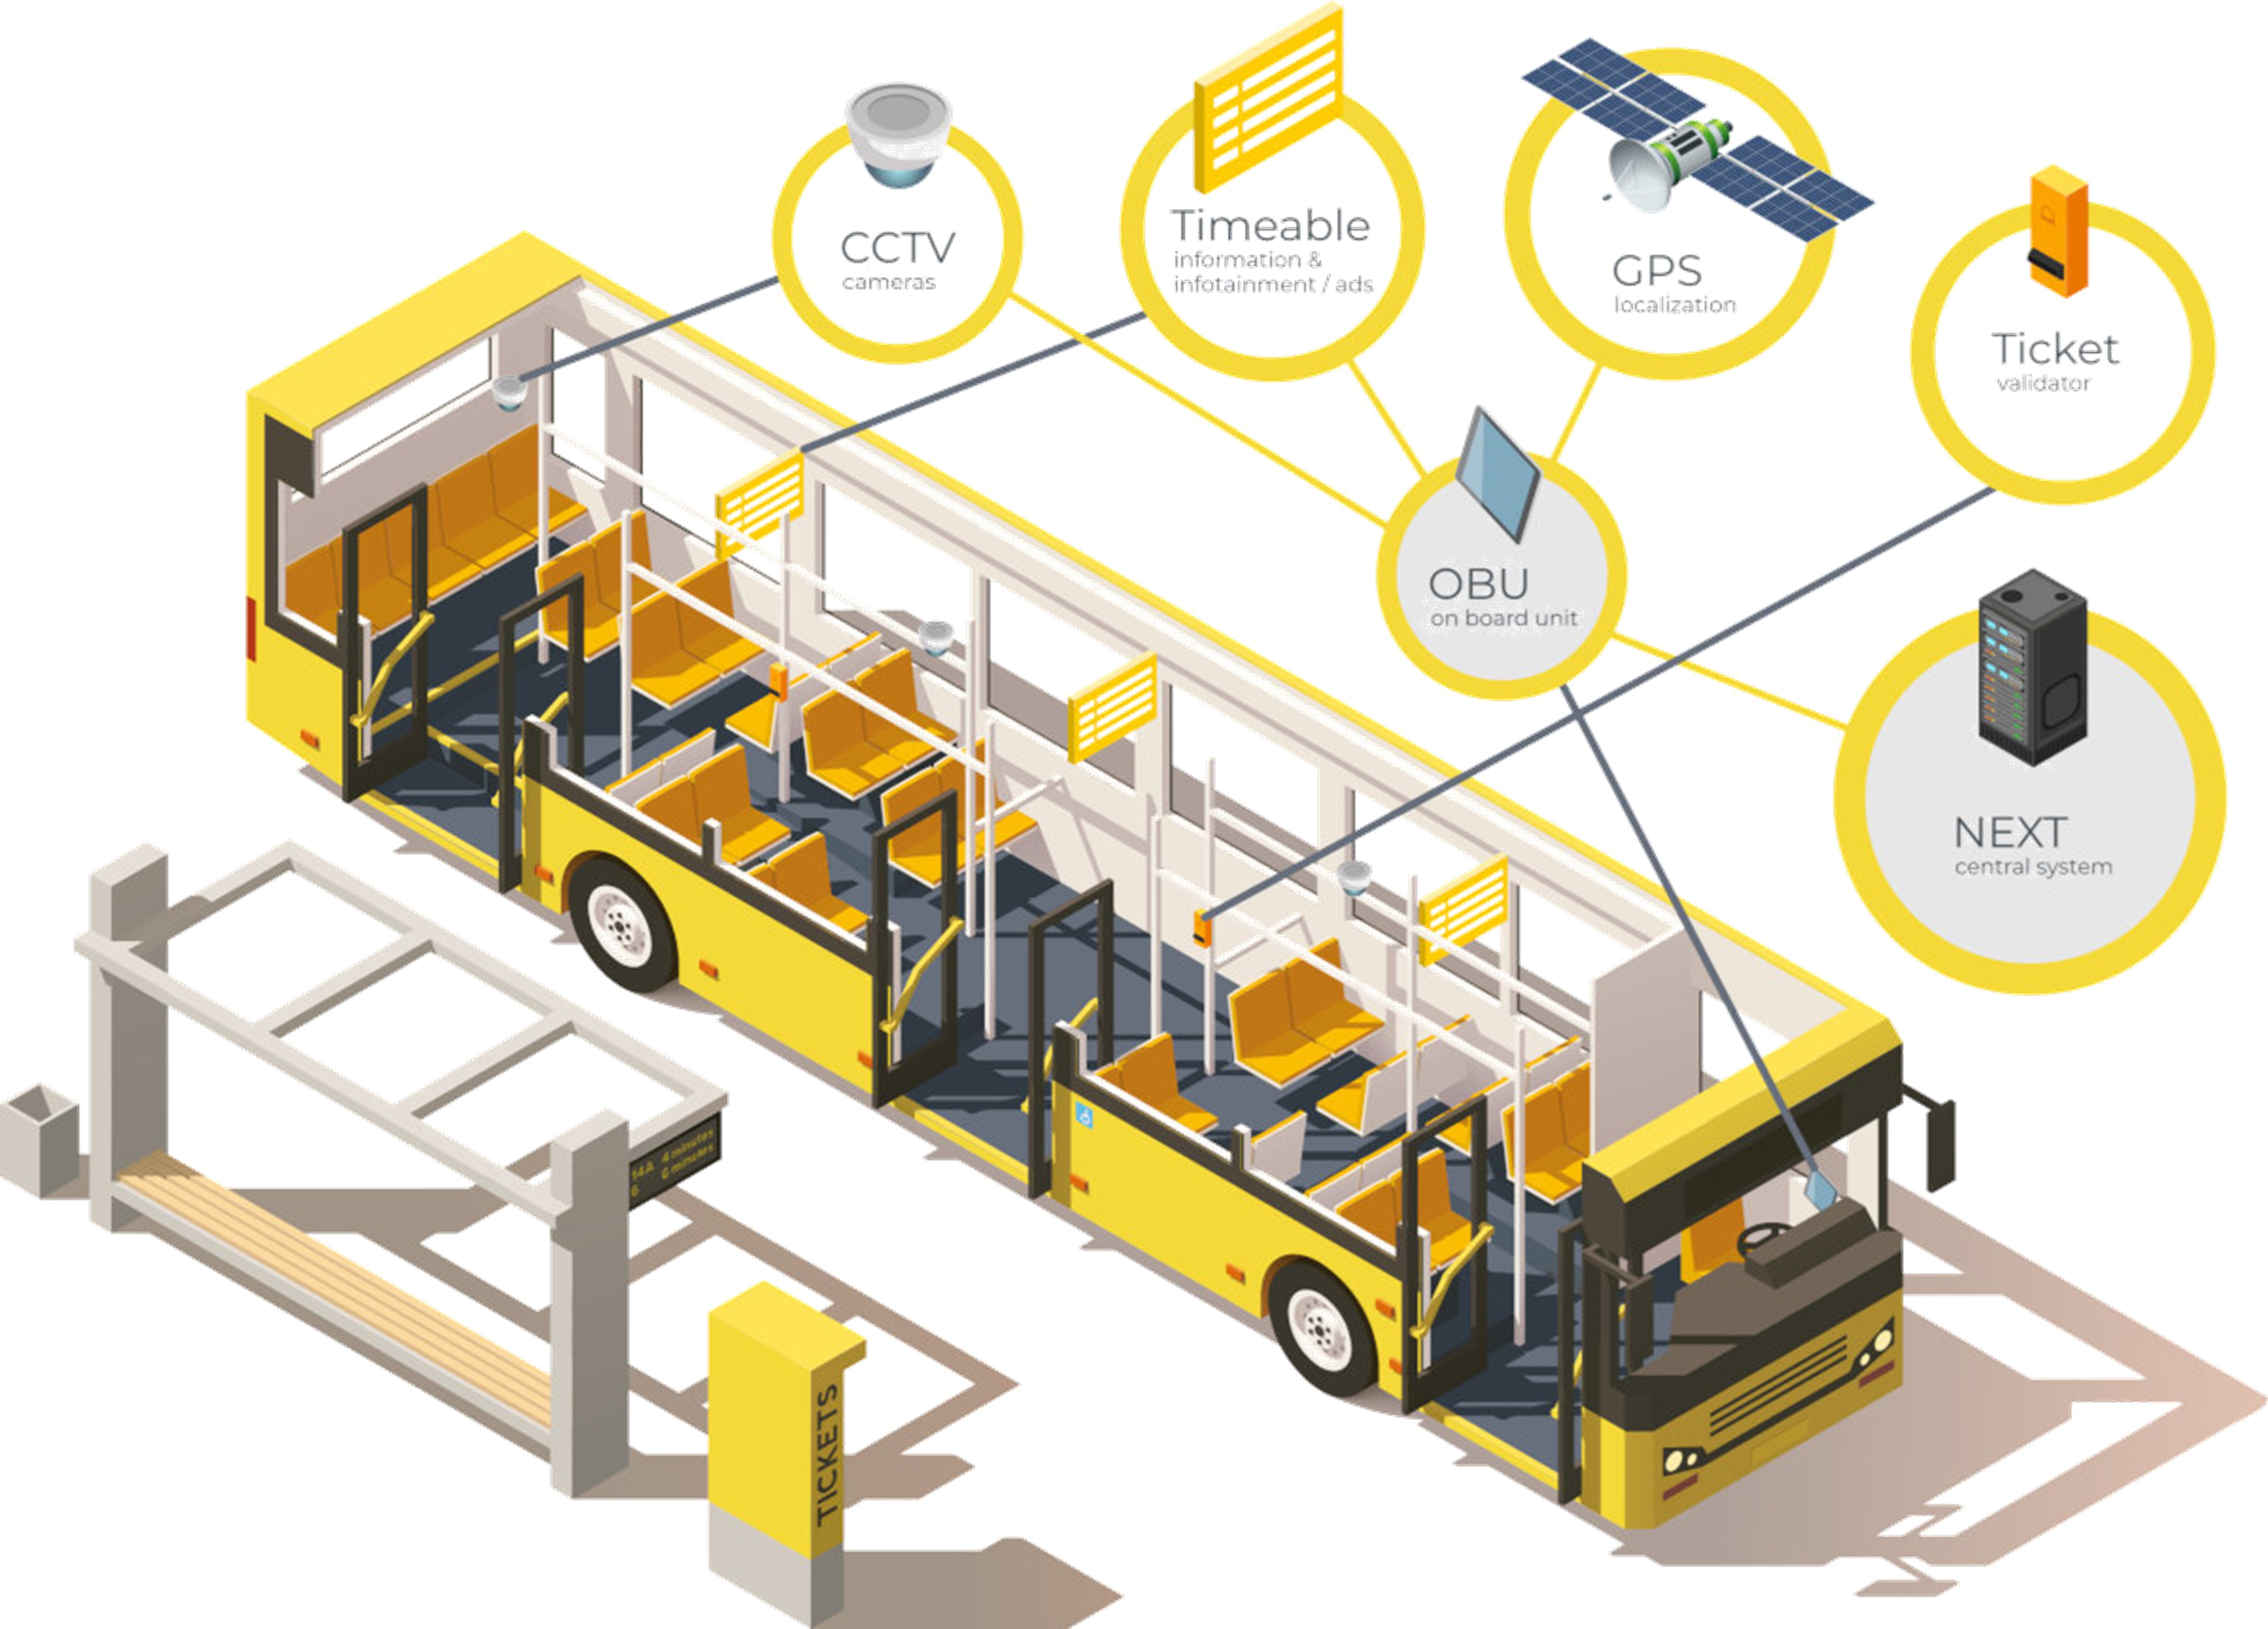
\includegraphics[width=0.7\textwidth]{Images/New Technologies/AVMeAVL.jpg}
    \caption{AVM and AVL\cite{avmavlimmage}}
    \label{fig:avmavl}
\end{figure}

\paragraph{Automatic People Counter}
People counters are electronic sensors that count people as they walk into an entrance. There are various methods for those systems to count people. Those can be classified into contact-type counters, sensors implemented system, and vision-based system using a camera. Contact-type counters are mechanical counters which need human contact such as turnstiles and mat-type foot switches that can obstruct the path. 

However, this type of counter only applicable for minimal people counting and it is not suitable for massive number of people, such as a high flow of people boarding or getting off the bus. Other technologies used in people counter are Pyroelectric Infrared (PIR) sensors, ultrasonic sound distance sensor and thermal sensor. PIR sensor counts people when they pass through the area of observation which is mounted with a pair of IR transceiver. Thermal sensors are only able to observe the crowd density without counting them accurately. 

\begin{figure}[h!]
    \centering
    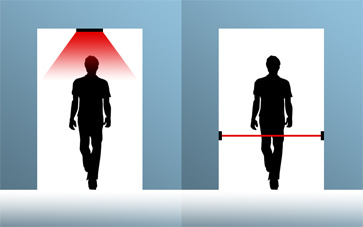
\includegraphics[width=0.5\textwidth]{Images/New Technologies/APC.jpg}
    \caption{Automatic People Counter\cite{apcimage}}
    \label{fig:APC}
\end{figure}

People counting technologies can be used for many purposes: assessing that is impossible to have them on all the lines of the consortium, it is possible to use a data analysis on routes that do not have APC to build a model to estimate the level of service onboard on all routes. The load factor information is very useful to consult on a real-time dashboard, creating a trend of the number of people on board; in this way it is also possible to study the performance of the stops, as well as the lines, creating a set of KPIs that can function both as real-time  indicators and for decision-making at a future planning level.

\paragraph{Video–surveillance }
Video-surveillance is a technology that is extremely helpful for public transport management; cameras can be installed in three main positions: outdoor cameras, to monitor the surrounding scene and in particular the blind spots, indoor cameras, to monitor bus passengers, and driver cameras, to monitor the driver behaviour. All those images can be provided to the driver with clear images referring to these areas, which can then be displayed on special monitors to be installed on the driver's dashboard. 

With the new telecommunication technologies, like 4G and 5G, it can be performed a sort of edge computing through the help of video analysis with AI systems; these methods can lead to fast and responsive actions or adjustment that the drivers, or the employees in remote, can do. Artificial Intelligence algorithms can detect some risk factors for what concern the ride’s safety, such as tiredness, distraction, or irregular behaviour of the driver.

\begin{figure}[h!]
    \centering
    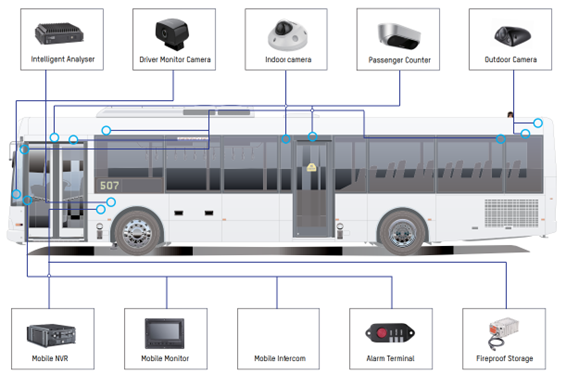
\includegraphics[width=0.6\textwidth]{Images/New Technologies/VIDEOSURV.PNG}
    \caption{Video–surveillance\cite{videosurvimage}}
    \label{fig:vs}
\end{figure}


\paragraph{Electronic ticketing systems}
The electronic ticketing system is not a proper technology installed just on buses, but the validation and control parts are managed largely on the bus. The system is composed by the validators and the On-Board Computer, which are installed directly on the buses, and by a central Control Center where all the data collection, management and distribution of incomes and emission or recharge of smart cards takes place.

\begin{figure}[h!]
    \centering
    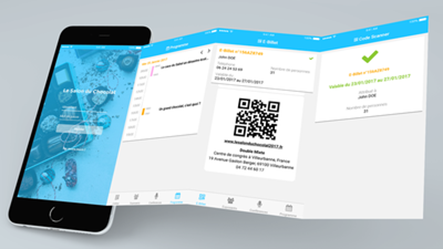
\includegraphics[width=0.45\textwidth]{Images/New Technologies/ELECTRONIC TICKET.png}
    \caption{Electronic ticketing systems\cite{eticketimage}}
    \label{fig:ets}
\end{figure}

One of the trending topics on the whole ticketing system is the type of support used: the support is the connection between costumers and PTO, which means that more information the support can bring to the PTO the better it is. In recent times there has been a rapid evolution of the support type, starting from basic paper, passing through magnetic, smart-cards and lastly mobile tickets. With Near-Field Communication (NFC) technology, the fares are redeemed without contact and completely remove the need to handle any physical cash or fares, and even limit the interaction needed with the driver. An additional motivation is that it is been found that physical money can carry the virus (in particular Covid-19) for up to three days, and by bypassing the need to purchase paper tickets and validate them, mobile ticketing can help reduce the transmission of the virus between riders and staff. An incredible by-product of integrating this technology is also the impact it has on the environment, as physical tickets no longer need to be created.

Keeping the user in mind, public transit technology is moving toward creating a more personalized ridership experience. A shift in this space is Account-Based Automatic Fare Collection. Through this system, all travel history, documents, and account information for riders is gathered in a customized dashboard.

With this technology, passengers can identify and participate with every available public service that is enabled for Account-based fare collection, making it far easier to use different modes of transportation, and save specific routes or journeys for use later. This also removes the hassle of having to manage multiple user accounts, payment methods, and receipt/billing information.

\subsection{Technologies installed off bus}
\label{subsec:techoffbus}
In addition to technologies directly installed on buses, there are some systems that play a center role in the world of public transport innovation, even not being directly on the public transport vehicle. Those type of technologies are aimed more at the network part of the service: we are talking about all the secondary, or subsidiary, technology that are vastly growing in the world, that together form the infamous Internet of Things. 

The general concept is that public transportation is affected by countless variables and not only by the ones directly connected to it, such as the costumers, the bus health, the drivers and so on, for example: the weather is clearly a source of data in correlation, but more importantly in causation, with the transportation system, if a day there is a particularly heavy rain, people tend to use more the private vehicle, using less the bus or in general the public transportation, this is due to the fact that often using PT means waiting outside under the rain. This situation have a great impact on the PTO systems, in fact bus tend to be less populated, so all the KPIs related to the number of costumers onboard are affected, as well as the travel time since, as said before, there are more private vehicles on the road than in a normal day; travel time therefore will be higher than usual and more delays, all of this affect the KPIs related to the commercial speed, travel time, delays per day and so on \dots

This big example is made to understand that the more data of different types are gathered daily, the more precise the analysis that a PTO can assess. In this new era of technology, especially now with the faster growing 5G, it is very important to take advantage of them, exploiting all of their potentialities.

The potential of digital applications and solutions for public transit is endless. Sensing devices and IoT technology are becoming more robust and low-cost, providing useful data for municipalities, fleet managers and even riders. For example, in Sweden a recent study used wireless sensors on city buses to monitor real-time air pollution. The sensors gave more accurate data on highly polluted urban areas, which led to better-informed city planning decisions and air quality improvement efforts. 

Telematics technology is also becoming a way to provide transportation fleet managers with real-time data to help identify and address things like temperature control, fuel levels, optimal driving routes, operating efficiencies and more. Predictive analytics allows for quick maintenance and better energy management, which is critical to addressing environmental impact.

Other important aspects on this topic are the actions that the PTA can take directly, for example, with the spread of smart cities, the necessary information and communication infrastructure lends itself well to intelligent traffic management systems. These systems allow centralised traffic control, enabling transit authorities to intelligently manage traffic lights, cameras, emergency routes and public transport routes.

Urban transit systems are also looking into how to incorporate rapid transit into existing systems. While this term most often refers to rapid transit trains or hyperloop systems, this can also refer to rapid transit buses, which have dedicated traffic lanes and priority at intersections; something that smart traffic management could help manage.


\subsection{New KPIs possibilities}
\label{subsec:newpossibilities}
As we have understood in the previous paragraphs, frequency in data–gathering is a key factor. Looking at the data provided to us is almost surprising that a company like Arriva, and all the consortium in general, has such a lack of detail in the available data. The dashboard built in the previous chapter has a potential, clearly limited by the frequency and the quality of what’s inside.

But why a higher frequency data – gathering is the base answer to most of the problems? Gathering more data more frequently means that it becomes much easier to understand trends, seasonalities, or particular micro – behavior that a monthly, or in some cases even yearly frequency cannot pick. In particular, algorithms like regression, classification, clustering, anomaly detection, and many others, work so much better with large quantities of data, and therefore understanding what they have to tell us is far easier.

Another strong motivation for why is essential to have data gathered more frequently is the possibility of expansion of the analysis that can be done: looking at a more detailed time span is useful to build a model on different types of time centered analysis, such as workdays vs. weekdays, peak hour vs. off-peak hours. The possibilities of Arriva, as now, are to compute KPIs based on the company trend of the month or year, which can hide an enormous quantity of information; having daily, hourly, or even more precise data, allows the analysts, and us, to build a dashboard with better KPIs.

\paragraph{Dynamic KPIs}
Other than more precise KPIs, gathering all those types of data can mean also being able to compute different \textit{types} of KPIs: we are used to looking at dashboards with basic cardinal numbers, which by definition are static and provide agglomerative information on the subject, such as a mean, a median, maximum or minimum and so on. 

Introducing the use of \textit{Dynamic KPIs} opens up a new dimension in the data – plane in which the analyst can look and assess more types of conclusions. The Dynamic KPI is a particular way to view a result where the user can look directly at the trend, in real-time of the data, but let’s make an example.

If we want to analyze the number of passengers onboard on a specific ride, until now the KPIs were all built as a mean number of the occupation onboard, representing the average number of passengers on that ride. But this information, which is still useful, don’t get us wrong, is not able to tell the users how the flow of passengers distributes among the stops of the ride. Using a dynamic KPIs that shows both the people loaded and unloaded at every stop, we can see in the data more information, such as a particular section in the run where there are very few people onboard, and if it is behavior repeated in time, this information is useful to assess some conclusion, such as remove some stops, add new ones and many more.

\begin{figure}[t]
    \centering
    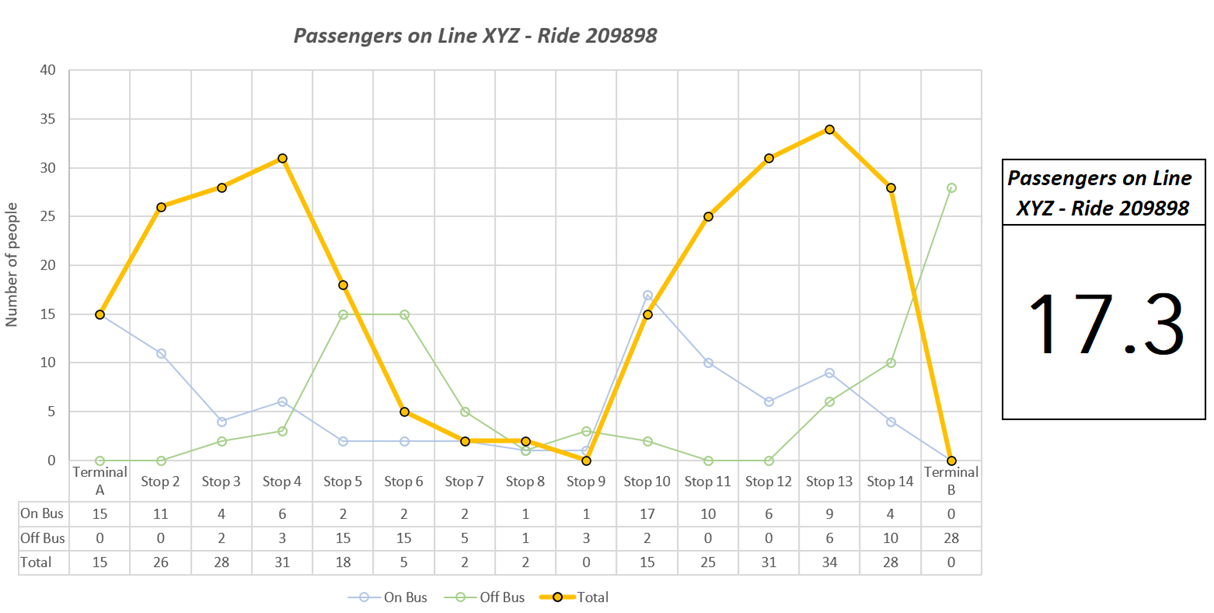
\includegraphics[width=1\textwidth]{Images/New Technologies/dynamic KPIs.png}
    \caption{Dynamic KPIs Example}
    \label{fig:dynKPI}
\end{figure}

As it is possible to see from the image  \ref{fig:dynKPI}, both are telling the same information, but in two different ways: the number on the right tells us just the mean number of passengers for that particular ride, although looking at the graph on the left we can detect much more information: the central stops of the ride (7, 8 and 9) are very little used, and also the number of passengers on board at that moment are almost zero. Here the PTO can make multiple decisions, such as dividing the line into two pieces to maximize the effectiveness of both of them. A deeper analysis can be done to understand why those stops are rarely used, maybe they can be re-positioned to meet higher demand, changing the line route by a little.




% Please add the following required packages to your document preamble:
% \usepackage{lscape}
%\newpage
\thispagestyle{empty}
%\begin{landscape}
\subsection{New Technologies KPIs examples}
\label{subsec:newKPIex}
Having know all the knowledge of new technologies that can be installed on and off the buses and all the new process that are involved to built more interesting KPIs, it is time to make some example, directly related to which data has Arriva now and what it could have in the future. In order to maintain the same scheme of pages in the traditional dashboard in \ref{ch:dashboard}, the KPIs are listed in the same structure:

\begin{table}[H]
\centering
\begin{tabular}{|l|l|l|l|}
\hline
\rowcolor{bluepoli!40}
\multicolumn{1}{|c|}{\textbf{KPI denomination}}                                       & \multicolumn{1}{c|}{\textbf{Technologies Used}} & \multicolumn{1}{c|}{\textbf{UoM}} & \multicolumn{1}{c|}{\textbf{Explanation}}                                                                                                                                                          \\ \hline
\begin{tabular}[c]{@{}l@{}}Daily single tickets   \\ sold over passenger \\ moved\end{tabular}  & Iot, E-Ticketing,   APC                & \begin{tabular}[c]{@{}l@{}} €\\ \ \# people \end{tabular}                                & \begin{tabular}[c]{@{}l@{}}Understand how\\ the amount \\ of single ticket sold affect \\ the overall passenger,\\  helping to size the service   \\ not only on historical \\ data and passes\end{tabular} \\ \hline
\begin{tabular}[c]{@{}l@{}}Distribution of   \\ ticket vs. pass per ride\end{tabular} & E-Ticketing, APC                     & \%                                            & \begin{tabular}[c]{@{}l@{}}Understand which   \\ type of costumer takes \\ certain rides allow to\\  assess decision for a ride\end{tabular}                                                       \\ \hline
\begin{tabular}[c]{@{}l@{}}Annual Fuel cost  \\  over km done\end{tabular}            & AVM, AVL                                        & €/km                                          & \begin{tabular}[c]{@{}l@{}}Helps understand the \\   driving behavior \\of the drivers \\ and the cost percentage \\ that affect \\the   balance sheets\end{tabular}                                   \\ \hline
\end{tabular}
\caption{List of new Economical and Financial KPIs}
\label{tab:economic}
\end{table}
%\end{landscape}
\newpage
% Please add the following required packages to your document preamble:
% \usepackage{lscape}
\newpage
\thispagestyle{empty}
\begin{landscape}
\begin{table}
\centering
\begin{tabular}{|l|l|l|l|}
\hline
\rowcolor{bluepoli!40}
\multicolumn{1}{|c|}{\textbf{KPI denomination}}                                                    & \multicolumn{1}{c|}{\textbf{\begin{tabular}[c]{@{}c@{}}Technologies \\ Used\end{tabular}}} & \multicolumn{1}{c|}{\textbf{\begin{tabular}[c]{@{}c@{}}Unit of\\  Measure\end{tabular}}} & \multicolumn{1}{c|}{\textbf{Explanation}}                                                                                                                                                        \\ \hline
\begin{tabular}[c]{@{}l@{}}Mean delay by time slot \\ (peak vs. off-peak) and ride\end{tabular}    & AVL, AVM                                                                                   & min                                                                                      & \begin{tabular}[c]{@{}l@{}}Understanding if a  \\delay is mainly caused \\ by the departing hour of the ride, \\ can help to modify   the schedule according to it\end{tabular}                    \\ \hline
\begin{tabular}[c]{@{}l@{}}Visualization on where \\ the ride generates the delay\end{tabular}     & AVL, AVM                                                                                   & map                                                                                      & \begin{tabular}[c]{@{}l@{}}Deepening the   knowledge of the delay \\ can mean even \\better improvements \\ going to make specific   changes \\ in some section of the lines\end{tabular}          \\ \hline
Lost costumers per   suppressed ride                                                               & APC, AVM                                                                                   & \#                                                                                       & \begin{tabular}[c]{@{}l@{}}Knowing how many   \\people are affected \\ by a suppressed ride\\ can help to assess \\ the importance of   that ride and an overall \\ level of discomfort\end{tabular} \\ \hline
Delay amount over mm   of rain                                                                     & AVM, IoT                                                                                   & min/mm                                                                                   & \begin{tabular}[c]{@{}l@{}}Knowing the relation  \\ between delays and \\ weather conditions\\ is important to correctly \\ dimension the   problem\end{tabular}                                     \\ \hline
\begin{tabular}[c]{@{}l@{}}Load Factor per run   \\ per time slot (peak vs. off-peak)\end{tabular} & APC, AVM                                                                                   & \%                                                                                       & \begin{tabular}[c]{@{}l@{}}Knowing the   percentage of load\\  for a particular run can help to allocate \\ better the resources\end{tabular}                                                    \\ \hline
Load Factor vs.   Weather Condition                                                                & APC, IoT                                                                                   & \%                                                                                       & \begin{tabular}[c]{@{}l@{}}Also in this case, knowing \\   the behavior in\\ different weather condition \\ can help to allocate better the resources\end{tabular}                                 \\ \hline
\end{tabular}
\caption{List of new Service Quality KPIs}
\label{tab:servicequality}
\end{table}
\end{landscape}
% Please add the following required packages to your document preamble:
% \usepackage[normalem]{ulem}
% \useunder{\uline}{\ul}{}
% \usepackage{lscape}
\newpage
\thispagestyle{empty}
\begin{landscape}
\begin{table}[]
\centering
\begin{tabular}{|l|l|l|l|}
\hline
\rowcolor{bluepoli!40}
\multicolumn{1}{|c|}{\textbf{KPI denomination}}                                                        & \multicolumn{1}{c|}{\textbf{Technologies Used}} & \multicolumn{1}{c|}{\textbf{Unit of Measure}} & \multicolumn{1}{c|}{\textbf{Explanation}}                                                                                                                                                                                                                             \\ \hline
\begin{tabular}[c]{@{}l@{}}Percentage of low environmental   \\ impact bus on the road\end{tabular}    & AVM                                             & \%                                            & \begin{tabular}[c]{@{}l@{}}Knowing how many green   bus \\ are circulating on the road can be \\ an interesting KPI to show at the PTA\end{tabular}                                                                                                                   \\ \hline
Percentage of km   made by hybrid/EV bus                                                               & AVM, AVL                                        & \%                                            & \begin{tabular}[c]{@{}l@{}}Same as before, knowing  how many kms \\ have been done in a healthy way is useful\end{tabular}                                                                                                                                            \\ \hline
Tons of $CO_2$ emitted   by bus or by line                                                             & AVM                                             & ton                                           & \begin{tabular}[c]{@{}l@{}}Understanding which   model of bus on which line\\  is the most emissive is useful to assess \\ how to renovate   the fleet\end{tabular}                                                                                                   \\ \hline
\begin{tabular}[c]{@{}l@{}}Tons of $CO_2$   \\ emitted in the city center vs. rural areas\end{tabular} & AVM, AVL                                        & ton                                           & \begin{tabular}[c]{@{}l@{}}Knowing the spatial   distribution of tonnage \\ emission can be useful to re-allocate different bus  \\  models on the lines\end{tabular}                                                                                                 \\ \hline
\begin{tabular}[c]{@{}l@{}}Mean bus consumption   \\ per run, per line, per bus type\end{tabular}      & AVL, AVM                                        & $L_{fuel}$/(run,   line, bus)                 & \begin{tabular}[c]{@{}l@{}}Awareness on bus   consumption by run is useful \\ to re-allocate and renovate the rolling stock\end{tabular}                                                                                                                              \\ \hline
Energy consumption curve   for EV bus                                                                  & AVM, AVL                                        & kWh/(time, km)                                & \begin{tabular}[c]{@{}l@{}}Having Electric Vehicle can be difficult to manage \\ in terms of recharging point and time allocation,  \\  understanding where the bus consume most \\ of its energy is handy to optimally   place \\ the recharging points\end{tabular} \\ \hline
\end{tabular}
\caption{List of new KPIs on Rolling Stock}
\label{tab:rollingstock}
\end{table}
\end{landscape}
% Please add the following required packages to your document preamble:
% \usepackage{lscape}
\newpage
\thispagestyle{empty}
% Please add the following required packages to your document preamble:
% \usepackage{lscape}
\begin{landscape}
\begin{table}[]
\centering
\begin{tabular}{|l|l|l|l|}
\hline
\rowcolor{bluepoli!40}
\multicolumn{1}{|c|}{\textbf{KPI denomination}}                                                       & \multicolumn{1}{c|}{\textbf{Technologies Used}} & \multicolumn{1}{c|}{\textbf{Unit of Measure}} & \multicolumn{1}{c|}{\textbf{Explanation}}                                                                                                                                                             \\ \hline
\begin{tabular}[c]{@{}l@{}}Commercial speed \\ deviation   from mean\end{tabular}                     & AVL, AVM, historical   data                     & $\pm$ km/h                                    & \begin{tabular}[c]{@{}l@{}}Comparing real-time   \\ commercial speed with the mean \\ of historical data help understand, \\ together   with delays information, \\ where is the problem\end{tabular} \\ \hline
Amount of km per day                                                                                  & AVM                                             & km                                            & Amount of kilometers   per day                                                                                                                                                                        \\ \hline
Planned vs. Effective   kms                                                                           & AVM                                             & \%                                            & \begin{tabular}[c]{@{}l@{}}Comparison between   \\ planned km on schedule \\ and km effectively done in a day\end{tabular}                                                                            \\ \hline
\begin{tabular}[c]{@{}l@{}}Mean time per stop   \\ (peak vs. off-peak)\end{tabular}                   & AVL                                             & sec                                           & \begin{tabular}[c]{@{}l@{}}Amount of time taken   at each stop to \\ loading and unloading the passengers\end{tabular}                                                                                \\ \hline
\begin{tabular}[c]{@{}l@{}}Stop time in   relation to number \\ of people moved per stop\end{tabular} & AVL, APC                                        & \# of people / sec                            & \begin{tabular}[c]{@{}l@{}}As the one above but    comparing it \\ to the number of people \\ that   actually moved\end{tabular}                                                                      \\ \hline
\begin{tabular}[c]{@{}l@{}}Commercial speed vs.\\ millimeters of rain/snow\end{tabular}               & AVL, IoT                                        & f(Km/h, mm)                                   & \begin{tabular}[c]{@{}l@{}}Comparison between mean  \\  commercial speed \\ of the ride and the amount \\ of rain fall in that period of   time\end{tabular}                                          \\ \hline
\begin{tabular}[c]{@{}l@{}}Commercial speed vs. \\ Fuel Consumption or $CO_2$ produced\end{tabular}   & AVL, AVM                                        & (km/h)/kWh, (km/h)/$tons_{CO\_2}$           & \begin{tabular}[c]{@{}l@{}}Helps understand the   driving behavior \\ of the drivers among with the points \\ where to optimize it\end{tabular}                                                       \\ \hline
\end{tabular}
\caption{List of new Operational KPIs}
\label{tab:operation_indication}
\end{table}
\end{landscape}

\subsection{Mock Up Dashboard}
The aim of this section is to built and visualize some mock-up dashboard pages, starting from the KPIs listed tables \ref{tab:economic}, \ref{tab:servicequality}, \ref{tab:rollingstock}, \ref{tab:operation_indication}.

We would like to point out that all pages are a mock-up also for what concerns the data present in he graphs, which may appear not close to the reality and made on purpose to talk about their benefits.

\newpage

\newpage
\begin{landscape}
\thispagestyle{empty}
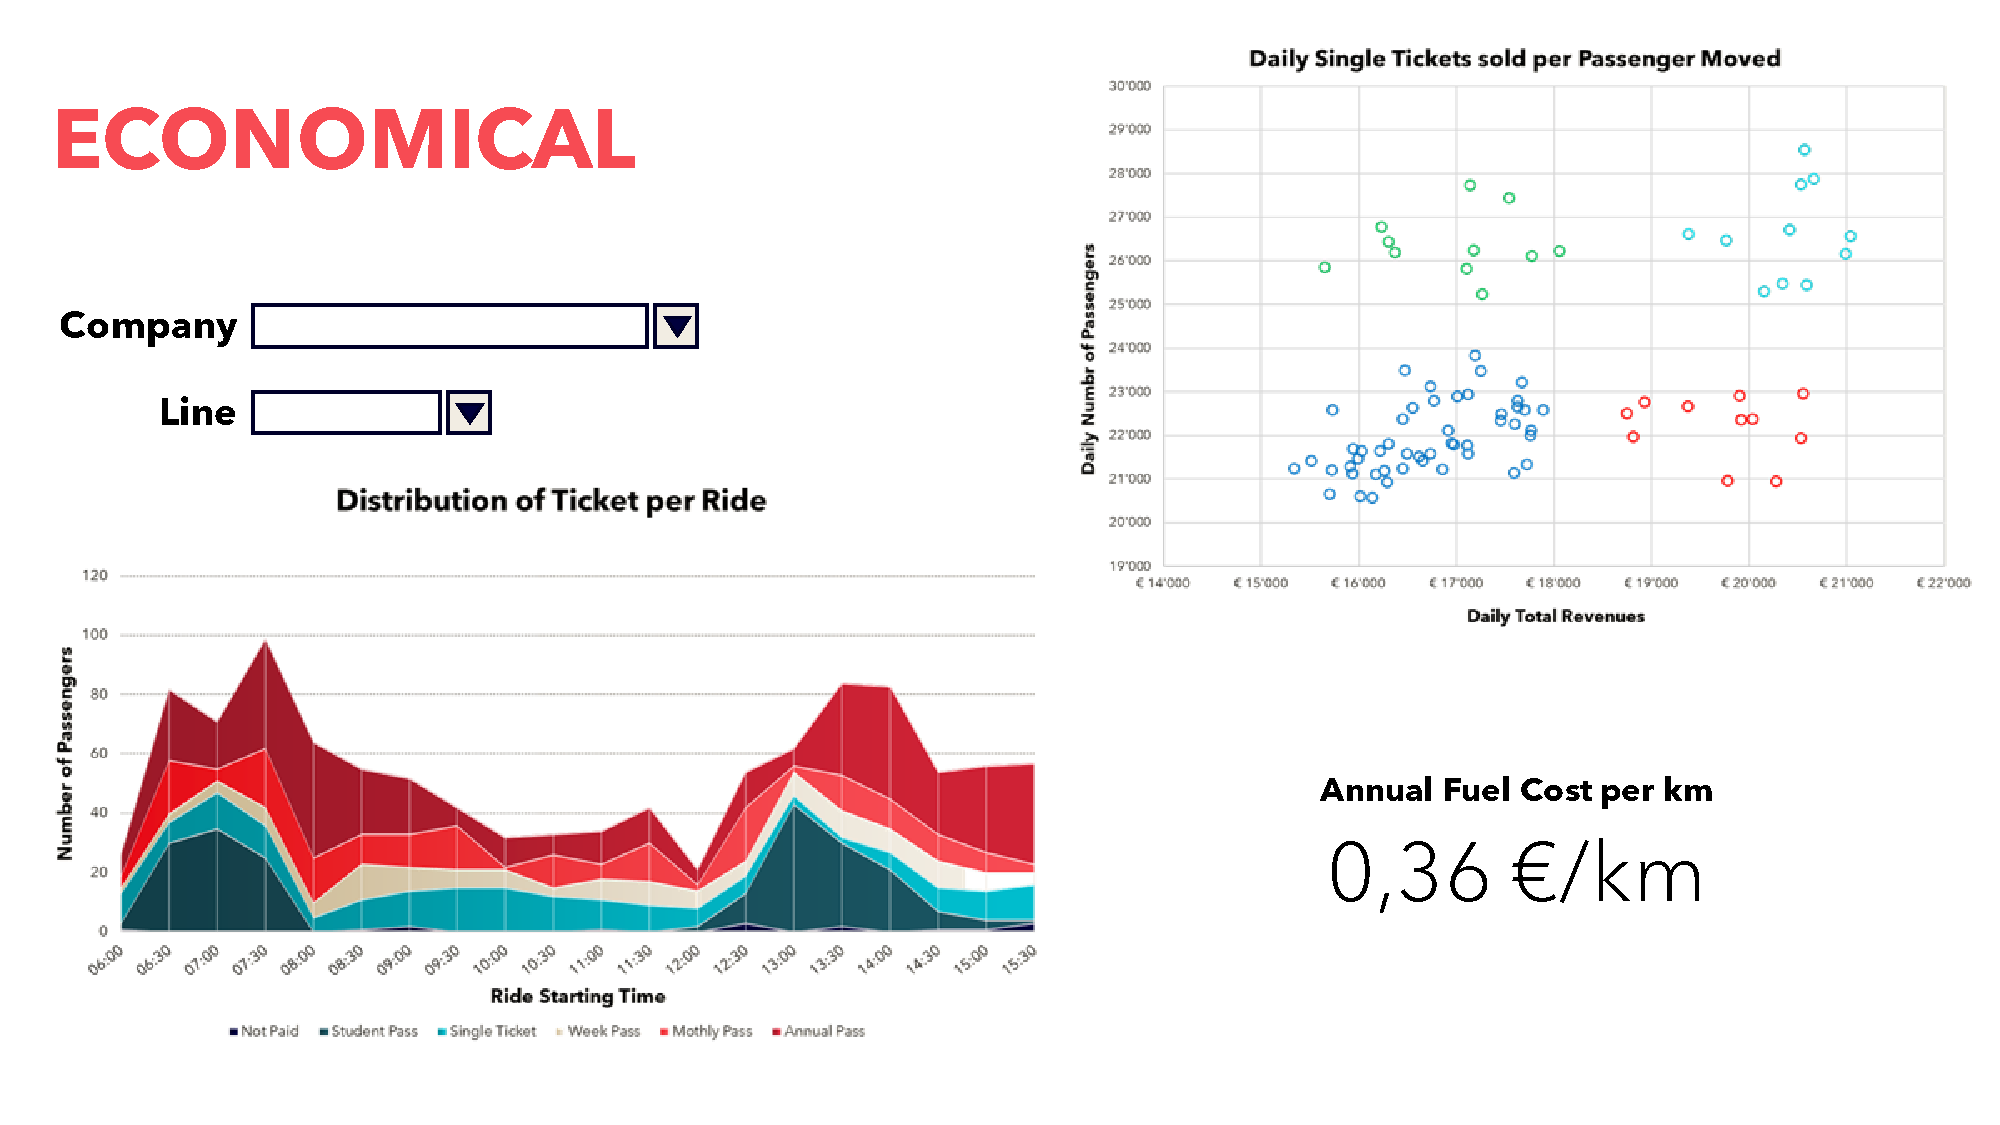
\includepdf[angle=90, pagecommand={\null\enlargethispage{3\baselineskip}\vfill\captionof{figure}{Economical page}\label{fig:ep}}]{mockup/economical.pdf}
\end{landscape}


\subsubsection{Economical page}
In this page we have created a visualization, in addition to the traditional one, able to tell a lot more information about the daily revenues of the company, for example, in the graph upright (\emph{Daily single tickets sold per passenger moved}) is possible to classify the dots (which each one represents a day) in four main areas:

\begin{itemize}
    \item \textcolor{blue}{\textbf{Blue Area}} is the normality, where average revenues are collected and the passengers moved are around a standard mean, depending, for example, from the day of the week of the time of the year.
    \item \textcolor{red}{\textbf{Red Area}} instead can represent the moment during the year where most people buy their monthly or yearly pass, which cause an abnormal amount of revenues, but still the passengers carried are quite constant.
    \item \textcolor{green}{\textbf{Green Area}} can be special day of the year, when maybe ticket office are closed (so less revenues from those), but a lot of people travel with public transport.
    \item \textcolor{cyan}{\textbf{Light Blue Area}} can represent some particular days when events happen, if Atalanta BC plays an important home game, a lot of supporters can choose to reach the stadium using public service, causing an substantial increase in the amount both in revenues and in passengers moved.
\end{itemize}

The graph in the lower-left part of the page shows the distribution of users of a particular line among its ride in the day. By visualizing how many people using different type of tickets have taken the bus, its possible to assess some actions regarding the advertising or the better sizing of the bus. So actions that can work on different levels: operational and marketing-wise.

\newpage
\begin{landscape}
\thispagestyle{empty}
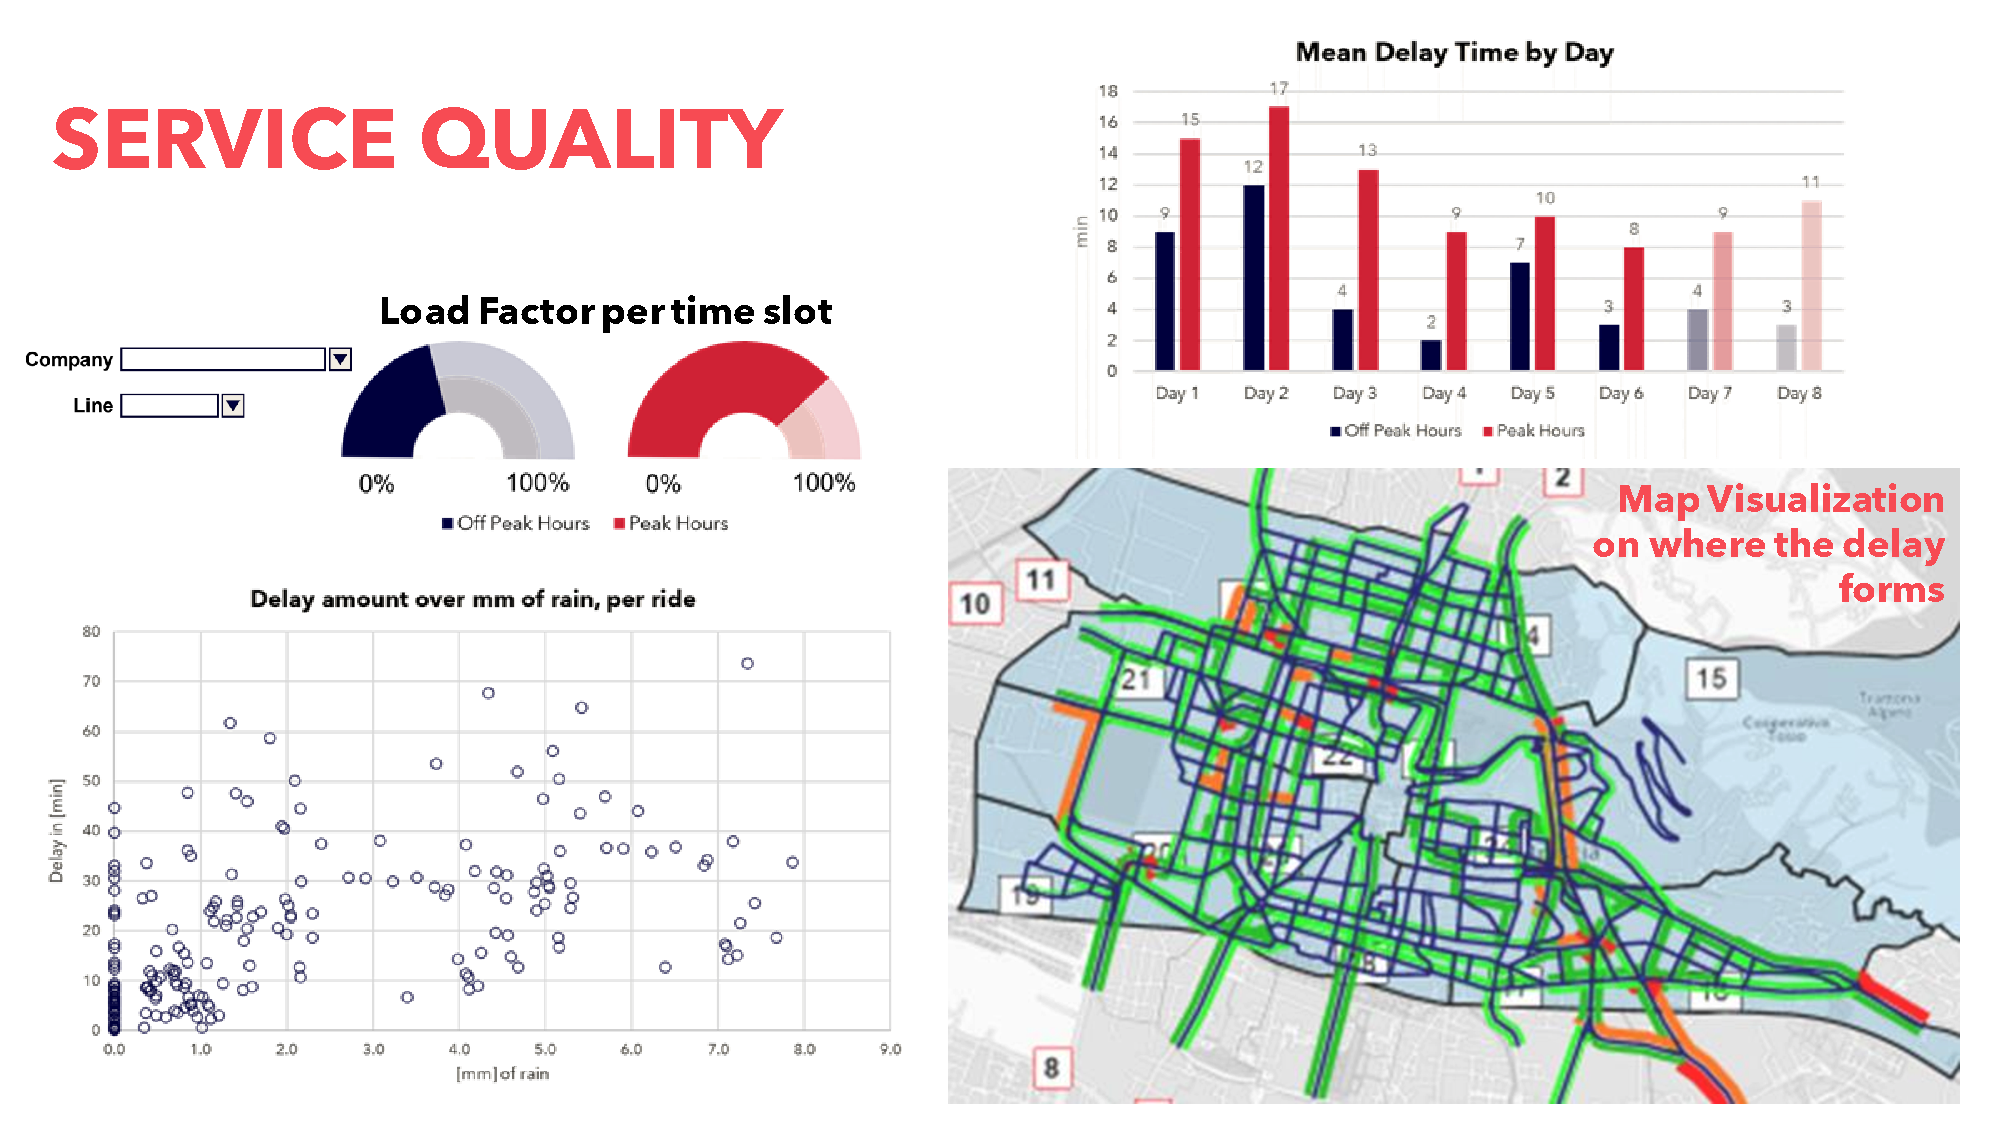
\includepdf[angle=90, pagecommand={\null\enlargethispage{3\baselineskip}\vfill\captionof{figure}{Service Quality page}\label{fig:sqp}}]{mockup/service_quality.pdf}
\end{landscape}

\subsubsection{Service Quality page}
Understanding the quality of service is a key factor both for the operational and economical side of the company, but also for the costumer satisfaction. Assessing its behavior daily can be a big help in order to understand all the minor actions in which the company can work on.

This page mainly focus on the \emph{delay} and its variablily taking into account:
\begin{itemize}
    \item Time of the Day: Peak and Off Peak Hours
    \item Weather Conditions: millimeters of rain (or snow)
    \item Location of the delay accumulation
\end{itemize}

Those three information together can help to visualize how and where the rides \emph{accumulate the delay}: knowing if there is a relation between minutes lost and millimeters of rain can, for example, help to a better planning on a day to day basis. Instead, for example, knowing \emph{where is located} the delay accumulation is useful to assess some major changes on the line path or work together with the PTA to find a more powerful solution.

\newpage
\begin{landscape}
\thispagestyle{empty}
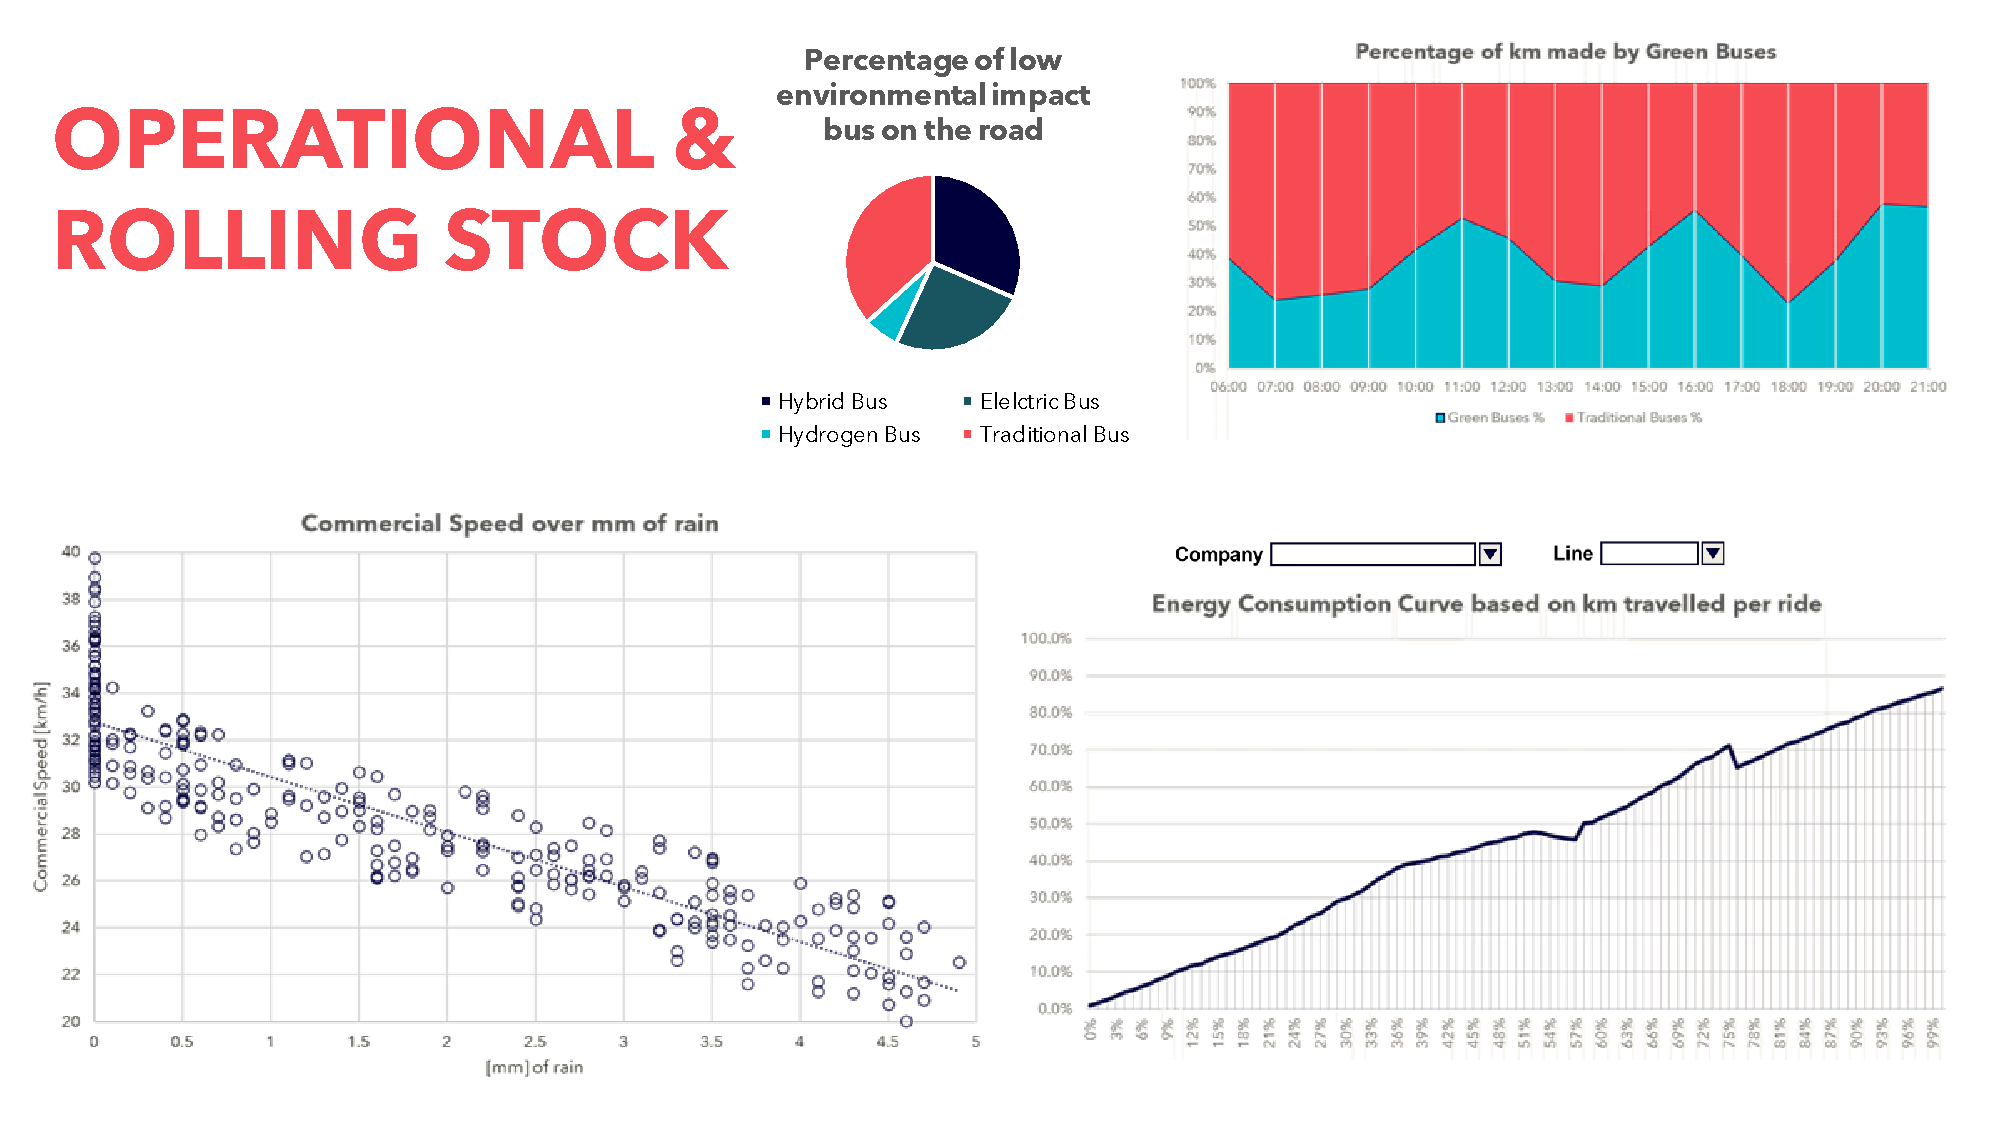
\includepdf[angle=90, pagecommand={\null\enlargethispage{3\baselineskip}\vfill\captionof{figure}{Rolling Stock and Operation page}\label{fig:sqp}}]{mockup/rolling_stock.pdf}
\end{landscape}

\subsubsection{Rolling Stock and Operation page}
This last page is more bus-centered, both looking at how the company is managing the fleet to be put on the road and assessing how well the fleet is performing looking at the Commercial Speed and the Energy Consumption curve.

The amount of green buses that a company have in their fleet is, and will be more and more, an important issue, we wanted to emphasize that by creating a visualization where is possible to know the percentage of Green Buses on road and with a visualization of the rolling stock composition.






